%   Filename    : chapter_4.tex 
\chapter{Preliminary Results/System Prototype}
\section{Data Gathering}
The data for dengue case prediction was gathered from a variety of reliable sources, enabling a comprehensive dataset spanning from January 2016 to September 2024. This dataset includes 452 rows of data, each containing weekly records of dengue cases along with corresponding meteorological variables, such as rainfall, temperature, and humidity.
\begin{enumerate}
	\item Dengue Case Data: The primary source of historical dengue cases came from the Humanitarian Data Exchange and the Western Visayas Center for Health Development (WVCHD). The dataset, accessed through Freedom of Information (FOI) requests, provided robust case numbers for the Western Visayas region. The systematic collection of these data points was essential for establishing a reliable baseline for model training and evaluation.
	\item Weather Data: Weekly weather data was obtained by web scraping from Weather Underground, allowing access to rainfall, temperature, and humidity levels that correlate with dengue prevalence.
\end{enumerate}

\begin{figure}[ht]
	\centering
	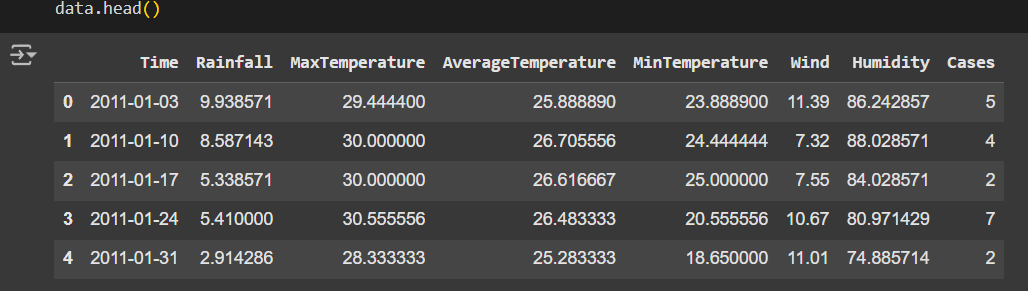
\includegraphics[width=0.75\textwidth]{data_snippet}
	\caption{Snippet of the Combined Dataset}
	\label{fig:data_snippet}
\end{figure}